\section{Estimated Speedup Using Amdahl's Law}\label{app:Amdahls}

%%%%%%%%%%%%%%%%%%%%%%

We estimated Amdahl's Law on the 3DM benchmark on DUT 2, which required us to know the parallelizable part of the benchmark. The parallelizable part had to be estimated because we did not have the source code for the benchmark. Each measurement starts with a period where the system is idle, then 3DM executes, followed by another period of the DUT being idle. We assumed that the period where 3DM is executed is the parallelizable part of the whole measurement, while the periods before and after are serial. Based on this assumption, we gathered estimates of the parallelizable and serial parts of the measurement. Then we computed the estimated speedup and compared it with the actual speedup.

\begin{figure}[H]
    \centering
    \begin{subfigure}[t]{0.4\textwidth}
        \centering
        %\begin{figure}[H]
    \begin{tikzpicture}
    \begin{axis}[
        title={Comparison of Speedup},
        xlabel={Number of Cores Used},
        ylabel={Speedup},
        xmin=1, xmax=10,
        ymin=0, ymax=4,
        xtick={1,2,3,4,5,6,7,8,9,10},
        ytick={0,1,2,3,4},
        legend pos=south east,
        ymajorgrids=true,
        grid style=dashed,
    ]
    
    \addplot[
        color=blue,
        mark=square,
        ]
        coordinates {
        (1,1)(2,1.6787346222)(3,2.1695941855)(4,2.5411013569)(5,2.8320683114)(6,3.0661245456)(7,3.2584795325)(8,3.4193663866)(9,3.5559232301)(10,3.6732810342)
        };
        \addlegendentry{Amdahl's Estimated Speedup}
    
    \addplot[
        color=red,
        mark=triangle,
        ]
        coordinates {
        (1,1)(2,1.5877659574)(3,2.1663138796)(4,2.4100925147)(5,2.7799767171)(6,2.9139719341)(7,2.8182533438)(8,2.9390769231)(9,2.9818938606)(10,2.9139719341)
        };
        \addlegendentry{Actual Speedup}
    
    \end{axis}
    \end{tikzpicture}
    \caption{A comparison on the estimated speedup from Amdahl's law and the actual Speedup for 3DM on DUT 2}\label{fig:amdahls}
%\end{figure}

    \end{subfigure}
    %\hfill
    \hspace{2cm}
    \begin{subfigure}[t]{0.4\textwidth}
        \centering
        \begin{figure}[H]
    \begin{tikzpicture}
    \begin{axis}[
        title={Average Watts},
        xlabel={Number of Cores Used},
        ylabel={Watts},
        xmin=1, xmax=10,
        ymin=0, ymax=15,
        xtick={1,2,3,4,5,6,7,8,9,10},
        ytick={0,1,2,3,4,5,6,7,8,9,10,11,12,13,14,15},
        legend pos=south east,
        ymajorgrids=true,
        grid style=dashed,
    ]
    
    \addplot[
        color=red,
        mark=triangle,
        ]
        coordinates {
        (1,8.8602320355)(2,10.6834482051)(3,11.7731373773)(4,12.5237974684)(5,13.0511557926)(6,13.3956136651)(7,13.5673410405)(8,13.6624354244)(9,13.6733193277)(10,13.4713951745)
        };
        \addlegendentry{Average Watts}
    
    \end{axis}
    \end{tikzpicture}
    \caption{Average watts for 3DM on DUT 2}\label{fig:amdahlsAveWat}
\end{figure}

    \end{subfigure}
    \caption{Speedup up and Average Watts for DUT2 on 3DM}
\end{figure}
%%\begin{figure}[H]
    \begin{tikzpicture}
    \begin{axis}[
        title={Comparison of Speedup},
        xlabel={Number of Cores Used},
        ylabel={Speedup},
        xmin=1, xmax=10,
        ymin=0, ymax=4,
        xtick={1,2,3,4,5,6,7,8,9,10},
        ytick={0,1,2,3,4},
        legend pos=south east,
        ymajorgrids=true,
        grid style=dashed,
    ]
    
    \addplot[
        color=blue,
        mark=square,
        ]
        coordinates {
        (1,1)(2,1.6787346222)(3,2.1695941855)(4,2.5411013569)(5,2.8320683114)(6,3.0661245456)(7,3.2584795325)(8,3.4193663866)(9,3.5559232301)(10,3.6732810342)
        };
        \addlegendentry{Amdahl's Estimated Speedup}
    
    \addplot[
        color=red,
        mark=triangle,
        ]
        coordinates {
        (1,1)(2,1.5877659574)(3,2.1663138796)(4,2.4100925147)(5,2.7799767171)(6,2.9139719341)(7,2.8182533438)(8,2.9390769231)(9,2.9818938606)(10,2.9139719341)
        };
        \addlegendentry{Actual Speedup}
    
    \end{axis}
    \end{tikzpicture}
    \caption{A comparison on the estimated speedup from Amdahl's law and the actual Speedup for 3DM on DUT 2}\label{fig:amdahls}
%\end{figure}

%\begin{figure}[H]
    \begin{tikzpicture}
    \begin{axis}[
        title={Average Watts},
        xlabel={Number of Cores Used},
        ylabel={Watts},
        xmin=1, xmax=10,
        ymin=0, ymax=15,
        xtick={1,2,3,4,5,6,7,8,9,10},
        ytick={0,1,2,3,4,5,6,7,8,9,10,11,12,13,14,15},
        legend pos=south east,
        ymajorgrids=true,
        grid style=dashed,
    ]
    
    \addplot[
        color=red,
        mark=triangle,
        ]
        coordinates {
        (1,8.8602320355)(2,10.6834482051)(3,11.7731373773)(4,12.5237974684)(5,13.0511557926)(6,13.3956136651)(7,13.5673410405)(8,13.6624354244)(9,13.6733193277)(10,13.4713951745)
        };
        \addlegendentry{Average Watts}
    
    \end{axis}
    \end{tikzpicture}
    \caption{Average watts for 3DM on DUT 2}\label{fig:amdahlsAveWat}
\end{figure}


On \cref{fig:amdahls}, the estimated and actual speedup was illustrated at different amounts of cores. From using $1$-$6$ cores, the benchmark was executed using P-cores, while from $7$-$10$, progressively more E-cores were utilized. This can be observed as the estimated and actual speedup follows closely until the DUT uses the E-cores. It should be noted that Amdahl's law is not meant for asymmetric CPUs and, as such, does not account for the difference in computational power of the E-cores. The effect of this was that for $7$-$10$ cores, the estimated speedup did not follow the actual speedup. The actual speedup results showed that the E-cores could not contribute to speeding up the benchmark. On \cref{sub@fig:amdahlsAveWat}, it was illustrated that after six cores, the average watts increased slower than from 1 to 6 cores, while the E-cores did not provide a speedup on the benchmark, they also did not increase the energy consumption as much as the P-cores. 

%Another factor which may contribute to the stagnation is that the GPU could be the bottleneck. (Perhaps test this by using our GPU).

%\begin{figure}[H]
    \begin{tikzpicture}
    \begin{axis}[
        title={Comparison of Average Watts},
        xlabel={Cores},
        ylabel={Average Watts},
        xmin=1, xmax=10,
        ymin=0, ymax=6,
        xtick={1,2,3,4,5,6,7,8,9,10},
        ytick={0,1,2,3,4,5,6},
        legend pos=south east,
        ymajorgrids=true,
        grid style=dashed,
    ]
    
    \addplot[
        color=blue,
        mark=square,
        ]
        coordinates {
        (1,1)(2,1.7664400703)(3,2.3962949728)(4,2.9393806865)(5,3.4239136624)(6,3.8670725446)(7,4.2799146201)(8,4.6698793631)(9,5.0421561883)(10,5.4004753118)
        };
        \addlegendentry{Estimated Average Power Consumption}
    
    \addplot[
        color=red,
        mark=triangle,
        ]
        coordinates {
        (1,1)(2,1.5547204332)(3,1.8747025475)(4,2.1087442671)(5,2.2675326631)(6,2.3413453141)(7,2.4091123316)(8,2.4388831154)(9,2.4406388005)(10,2.3710283913)
        };
        \addlegendentry{Actual Average Power Consumption}
    
    \end{axis}
    \end{tikzpicture}
    \caption{A comparison on the estimated average power consumption from Amdahl's extended law and the actual average power consumption for 3DM on DUT 2}\label{fig:amdahlsExt}
\end{figure}

%\begin{figure}[H]
    \begin{tikzpicture}
    \begin{axis}[
        title={Comparison of Perf/W},
        xlabel={Cores},
        ylabel={Perf/W},
        xmin=1, xmax=10,
        ymin=0, ymax=2,
        xtick={1,2,3,4,5,6,7,8,9,10},
        ytick={0,1,2},
        legend pos=south east,
        ymajorgrids=true,
        grid style=dashed,
    ]
    
    \addplot[
        color=blue,
        mark=square,
        ]
        coordinates {
        (1,1)(2,0.9503490384)(3,0.9053952915)(4,0.8645022976)(5,0.8271436113)(6,0.7928800172)(7,0.7613421813)(8,0.7322172846)(9,0.7052386117)(10,0.6801773589)
        };
        \addlegendentry{Estimated Perf/W}
    
    \addplot[
        color=red,
        mark=triangle,
        ]
        coordinates {
        (1,1)(2,1.0212549623)(3,1.1555507206)(4,1.1429041218)(5,1.2259919173)(6,1.2445716215)(7,1.1698306081)(8,1.2050913406)(9,1.2217677847)(10,1.2289907387)
        };
        \addlegendentry{Actual Perf/W}
    
    \end{axis}
    \end{tikzpicture}
    \caption{A comparison on the estimated Perf/W from Amdahl's extended law and the actual Perf/W for 3DM on DUT 2}\label{fig:amdahlsExtPerfW}
\end{figure}


% The extension of Amdahl's Law as described in \cref{woo2008extending} estimates average power consumption of each core by using a fraction for the power the processor uses in idle. 







%\begin{figure}[H]
    \centering
    \begin{tikzpicture}[]
        \pgfplotsset{
            width=0.9\textwidth,
            height=0.26\textheight
        }
        \begin{axis}[
            xlabel={Average Energy Consumption (Joules)}, 
            title={The energy consumption of the CPU}, 
            ytick={1, 2, 3, 4, 5, 6, 7, 8},
        yticklabels={
             0, 1, 2, 3, 4, 5, 6, 7,  0, 5, 6, 2, 4, 3, 1,  0, 5, 6, 2, 4, 3,  0, 5, 6, 2, 4,  0, 5, 6, 2,  0, 5, 6,  0, 5,  0
            },
            xmin=0,xmax=2000,
            ]
        
        
        \addplot+ [boxplot prepared={
                lower whisker=1600.59619140625,
                lower quartile=1645.1446228027344,
                median=1678.9347534179688,
                upper quartile=1707.7724914550781,
                upper whisker=1778.0560302734375
                }, color = red
                ] coordinates{(0,1836.4364013671875)(0,3873.498046875)(0,3791.6630859375)};
        
        \addplot+ [boxplot prepared={
                lower whisker=1640.5601806640625,
                lower quartile=1669.5162353515625,
                median=1702.5245971679688,
                upper quartile=1739.0556945800781,
                upper whisker=1838.66162109375
                }, color = red
                ] coordinates{(1,1943.2760009765625)(1,1864.127685546875)(1,3976.25732421875)(1,3849.386962890625)};
        
        \addplot+ [boxplot prepared={
                lower whisker=1666.2357177734375,
                lower quartile=1699.4358215332031,
                median=1735.8279418945312,
                upper quartile=1784.6516418457031,
                upper whisker=1889.923828125
                }, color = red
                ] coordinates{(2,1963.513427734375)(2,3960.526611328125)(2,3802.806884765625)};
        
        \addplot+ [boxplot prepared={
                lower whisker=1680.410888671875,
                lower quartile=1734.2084045410156,
                median=1772.0855102539062,
                upper quartile=1807.1498107910156,
                upper whisker=1891.77099609375
                }, color = red
                ] coordinates{(3,2009.88525390625)(3,4301.60595703125)(3,4157.505859375)};
        
        \addplot+ [boxplot prepared={
                lower whisker=1727.8282470703125,
                lower quartile=1767.1727294921875,
                median=1806.1300048828125,
                upper quartile=1846.2762145996094,
                upper whisker=1931.2103271484375
                }, color = red
                ] coordinates{(4,2098.440673828125)(4,1975.8546142578125)(4,4107.337890625)(4,4007.394775390625)};
        
        \addplot+ [boxplot prepared={
                lower whisker=1671.0252685546875,
                lower quartile=1717.2276611328125,
                median=1758.0728759765625,
                upper quartile=1798.5192260742188,
                upper whisker=1877.529052734375
                }, color = red
                ] coordinates{(5,2025.55615234375)(5,3929.595703125)(5,3796.85986328125)};
        
        \addplot+ [boxplot prepared={
                lower whisker=1837.3095703125,
                lower quartile=1886.635986328125,
                median=1941.7662353515625,
                upper quartile=1991.511962890625,
                upper whisker=2110.62841796875
                }, color = red
                ] coordinates{(6,2205.58740234375)(6,4366.18310546875)(6,4249.7890625)};
        
        \addplot+ [boxplot prepared={
                lower whisker=2317.460693359375,
                lower quartile=2388.1891479492188,
                median=2430.9105224609375,
                upper quartile=2510.6082153320312,
                upper whisker=2662.027587890625
                }, color = red
                ] coordinates{(7,2716.302001953125)};
        
        
        \end{axis}
    \end{tikzpicture}
\caption{CPU measurements by IPG on DUT 1 for test case(s) 3DM compiled on } \label{fig:3-same-mi-different-application-post-config-update-ipg-3d-mark.exe-unkown-workstationone-cpu-energy_consumption}
\end{figure}
%\begin{figure}[H]
    \centering
    \begin{tikzpicture}[]
        \pgfplotsset{
            width=0.9\textwidth,
            height=0.26\textheight
        }
        \begin{axis}[
            xlabel={Average Execution Time (s)}, 
            ylabel={Core}, 
            title={The Average Execution Time}, 
            ytick={1, 2, 3, 4, 5, 6, 7, 8},
        yticklabels={
             0,  1,  2,  3,  4,  5,  6,  7
            },
            xmin=0,xmax=60,
            ]
        
        
        \addplot+ [boxplot prepared={
                lower whisker=9.997,
                lower quartile=9.999,
                median=10.004,
                upper quartile=10.007,
                upper whisker=10.018
                }, color = red
                ] coordinates{(0,10.029)(0,10.031)(0,10.029)(0,10.03)(0,10.036)(0,10.022)(0,10.037)(0,10.05)(0,10.036)(0,10.051)(0,10.019)(0,10.034)(0,10.034)(0,10.037)(0,10.036)(0,10.02)(0,10.019)(0,10.019)(0,10.035)(0,10.038)(0,10.035)(0,10.033)(0,10.019)(0,10.021)(0,10.019)(0,10.035)(0,10.037)(0,10.02)(0,10.021)(0,10.019)(0,10.023)(0,10.05)(0,10.02)(0,10.019)(0,10.035)(0,10.035)(0,10.022)(0,10.02)(0,10.019)(0,10.034)(0,10.035)(0,10.052)(0,10.035)(0,10.035)(0,10.02)(0,10.036)(0,10.021)(0,10.02)(0,10.035)(0,10.02)(0,10.035)(0,10.021)(0,10.022)(0,10.051)(0,10.035)(0,10.036)(0,10.019)(0,10.035)(0,10.036)(0,10.02)(0,10.022)(0,10.019)(0,10.022)(0,10.037)(0,10.021)(0,10.02)(0,10.036)(0,10.035)(0,10.053)(0,10.022)(0,10.036)(0,10.019)(0,10.02)(0,10.02)(0,10.035)(0,10.021)(0,10.034)(0,10.02)(0,10.019)(0,10.066)(0,10.034)(0,10.033)(0,10.021)(0,10.021)(0,10.035)(0,10.02)(0,10.035)(0,10.037)(0,10.019)(0,10.035)};
        
        \addplot+ [boxplot prepared={
                lower whisker=9.988,
                lower quartile=9.996,
                median=10.002,
                upper quartile=10.004,
                upper whisker=10.012
                }, color = red
                ] coordinates{(1,10.108)(1,10.028)(1,10.027)(1,10.027)(1,10.046)(1,10.017)(1,10.033)(1,10.017)(1,10.019)(1,10.018)(1,10.081)(1,10.035)(1,10.018)(1,10.019)(1,10.017)(1,10.034)(1,10.017)(1,10.033)(1,10.02)(1,10.034)(1,10.017)(1,10.035)(1,10.019)(1,10.033)(1,10.018)(1,10.019)(1,10.017)(1,10.034)(1,10.017)(1,10.017)(1,10.082)(1,10.033)(1,10.019)(1,10.018)(1,10.037)(1,10.019)(1,10.017)(1,10.019)(1,10.021)(1,10.017)(1,10.032)(1,10.02)(1,10.019)(1,10.033)(1,10.032)(1,10.018)(1,10.034)(1,10.02)(1,10.018)(1,10.05)(1,10.017)(1,10.051)(1,10.035)};
        
        \addplot+ [boxplot prepared={
                lower whisker=9.986,
                lower quartile=9.995,
                median=10.001,
                upper quartile=10.002,
                upper whisker=10.011
                }, color = red
                ] coordinates{(2,10.027)(2,10.013)(2,10.016)(2,10.017)(2,10.032)(2,10.035)(2,10.047)(2,10.017)(2,10.047)(2,10.017)(2,10.017)(2,10.032)(2,10.032)(2,10.033)(2,10.015)(2,10.033)(2,10.032)(2,10.02)(2,10.034)(2,10.033)(2,10.018)(2,10.018)(2,10.065)(2,10.016)(2,10.031)(2,10.033)};
        
        \addplot+ [boxplot prepared={
                lower whisker=9.987,
                lower quartile=9.996,
                median=10.0,
                upper quartile=10.002,
                upper whisker=10.011
                }, color = red
                ] coordinates{(3,9.986)(3,10.012)(3,10.012)(3,10.018)(3,10.033)(3,10.016)(3,10.016)(3,10.033)(3,10.033)(3,10.018)(3,10.016)(3,10.016)(3,10.032)(3,10.033)(3,10.016)(3,10.017)(3,10.016)(3,10.08)(3,10.032)(3,10.017)(3,10.016)(3,10.015)(3,10.033)(3,10.017)};
        
        \addplot+ [boxplot prepared={
                lower whisker=9.987,
                lower quartile=9.996,
                median=10.001,
                upper quartile=10.002,
                upper whisker=10.011
                }, color = red
                ] coordinates{(4,10.028)(4,10.059)(4,10.027)(4,10.027)(4,10.033)(4,10.018)(4,10.018)(4,10.017)(4,10.016)(4,10.032)(4,10.032)(4,10.031)(4,10.016)(4,10.032)(4,10.017)(4,10.017)(4,10.017)(4,10.017)(4,10.018)(4,10.016)(4,10.017)(4,10.018)(4,10.032)(4,10.033)(4,10.031)(4,10.016)(4,10.018)(4,10.015)(4,10.017)(4,10.047)(4,10.048)(4,10.032)(4,10.031)(4,10.017)(4,10.017)};
        
        \addplot+ [boxplot prepared={
                lower whisker=9.988,
                lower quartile=9.995,
                median=10.001,
                upper quartile=10.002,
                upper whisker=10.011
                }, color = red
                ] coordinates{(5,10.215)(5,10.027)(5,10.026)(5,10.047)(5,10.017)(5,10.017)(5,10.047)(5,10.018)(5,10.033)(5,10.032)(5,10.031)(5,10.017)(5,10.016)(5,10.032)(5,10.017)(5,10.033)(5,10.033)(5,10.017)(5,10.018)(5,10.032)(5,10.017)(5,10.017)(5,10.032)(5,10.033)(5,10.017)(5,10.016)(5,10.033)(5,10.017)(5,10.017)};
        
        \addplot+ [boxplot prepared={
                lower whisker=9.987,
                lower quartile=9.995,
                median=10.000499999999999,
                upper quartile=10.002,
                upper whisker=10.011
                }, color = red
                ] coordinates{(6,10.018)(6,10.05)(6,10.017)(6,10.031)(6,10.018)(6,10.064)(6,10.018)(6,10.016)(6,10.019)(6,10.018)};
        
        \addplot+ [boxplot prepared={
                lower whisker=10.004,
                lower quartile=10.015,
                median=10.017,
                upper quartile=10.027,
                upper whisker=10.043
                }, color = red
                ] coordinates{(7,10.057)(7,10.058)(7,10.064)(7,10.048)(7,10.049)(7,10.047)};
        
        
        \end{axis}
    \end{tikzpicture}
\caption{Execution time measurements by IPG on DUT 1 for test case(s) NB compiled on oneAPI} \label{fig:3-same-one-api-compiler-different-cores-ipg-nbody.exe-intel-one-api-workstationone-runtime-duration}
\end{figure}

% \begin{figure}[H]
    \centering
    \begin{tikzpicture}[]
        \pgfplotsset{
            width=0.9\textwidth,
            height=0.26\textheight
        }
        \begin{axis}[
            xlabel={Average Energy Consumption (Joules)}, 
            title={The energy consumption of the CPU}, 
            ytick={1, 2, 3, 4, 5, 6, 7, 8},
        yticklabels={
             0, 1, 2, 3, 4, 5, 6, 7,  0, 5, 6, 2, 4, 3, 1,  0, 5, 6, 2, 4, 3,  0, 5, 6, 2, 4,  0, 5, 6, 2,  0, 5, 6,  0, 5,  0
            },
            xmin=0,xmax=2000,
            ]
        
        
        \addplot+ [boxplot prepared={
                lower whisker=1600.59619140625,
                lower quartile=1645.1446228027344,
                median=1678.9347534179688,
                upper quartile=1707.7724914550781,
                upper whisker=1778.0560302734375
                }, color = red
                ] coordinates{(0,1836.4364013671875)(0,3873.498046875)(0,3791.6630859375)};
        
        \addplot+ [boxplot prepared={
                lower whisker=1640.5601806640625,
                lower quartile=1669.5162353515625,
                median=1702.5245971679688,
                upper quartile=1739.0556945800781,
                upper whisker=1838.66162109375
                }, color = red
                ] coordinates{(1,1943.2760009765625)(1,1864.127685546875)(1,3976.25732421875)(1,3849.386962890625)};
        
        \addplot+ [boxplot prepared={
                lower whisker=1666.2357177734375,
                lower quartile=1699.4358215332031,
                median=1735.8279418945312,
                upper quartile=1784.6516418457031,
                upper whisker=1889.923828125
                }, color = red
                ] coordinates{(2,1963.513427734375)(2,3960.526611328125)(2,3802.806884765625)};
        
        \addplot+ [boxplot prepared={
                lower whisker=1680.410888671875,
                lower quartile=1734.2084045410156,
                median=1772.0855102539062,
                upper quartile=1807.1498107910156,
                upper whisker=1891.77099609375
                }, color = red
                ] coordinates{(3,2009.88525390625)(3,4301.60595703125)(3,4157.505859375)};
        
        \addplot+ [boxplot prepared={
                lower whisker=1727.8282470703125,
                lower quartile=1767.1727294921875,
                median=1806.1300048828125,
                upper quartile=1846.2762145996094,
                upper whisker=1931.2103271484375
                }, color = red
                ] coordinates{(4,2098.440673828125)(4,1975.8546142578125)(4,4107.337890625)(4,4007.394775390625)};
        
        \addplot+ [boxplot prepared={
                lower whisker=1671.0252685546875,
                lower quartile=1717.2276611328125,
                median=1758.0728759765625,
                upper quartile=1798.5192260742188,
                upper whisker=1877.529052734375
                }, color = red
                ] coordinates{(5,2025.55615234375)(5,3929.595703125)(5,3796.85986328125)};
        
        \addplot+ [boxplot prepared={
                lower whisker=1837.3095703125,
                lower quartile=1886.635986328125,
                median=1941.7662353515625,
                upper quartile=1991.511962890625,
                upper whisker=2110.62841796875
                }, color = red
                ] coordinates{(6,2205.58740234375)(6,4366.18310546875)(6,4249.7890625)};
        
        \addplot+ [boxplot prepared={
                lower whisker=2317.460693359375,
                lower quartile=2388.1891479492188,
                median=2430.9105224609375,
                upper quartile=2510.6082153320312,
                upper whisker=2662.027587890625
                }, color = red
                ] coordinates{(7,2716.302001953125)};
        
        
        \end{axis}
    \end{tikzpicture}
\caption{CPU measurements by IPG on DUT 1 for test case(s) 3DM compiled on } \label{fig:3-same-mi-different-application-post-config-update-ipg-3d-mark.exe-unkown-workstationone-cpu-energy_consumption}
\end{figure}
% \begin{figure}[H]
    \centering
    \begin{tikzpicture}[]
        \pgfplotsset{
            width=0.9\textwidth,
            height=0.26\textheight
        }
        \begin{axis}[
            xlabel={Average Execution Time (s)}, 
            ylabel={Core}, 
            title={The Average Execution Time}, 
            ytick={1, 2, 3, 4, 5, 6, 7, 8},
        yticklabels={
             0,  1,  2,  3,  4,  5,  6,  7
            },
            xmin=0,xmax=60,
            ]
        
        
        \addplot+ [boxplot prepared={
                lower whisker=9.997,
                lower quartile=9.999,
                median=10.004,
                upper quartile=10.007,
                upper whisker=10.018
                }, color = red
                ] coordinates{(0,10.029)(0,10.031)(0,10.029)(0,10.03)(0,10.036)(0,10.022)(0,10.037)(0,10.05)(0,10.036)(0,10.051)(0,10.019)(0,10.034)(0,10.034)(0,10.037)(0,10.036)(0,10.02)(0,10.019)(0,10.019)(0,10.035)(0,10.038)(0,10.035)(0,10.033)(0,10.019)(0,10.021)(0,10.019)(0,10.035)(0,10.037)(0,10.02)(0,10.021)(0,10.019)(0,10.023)(0,10.05)(0,10.02)(0,10.019)(0,10.035)(0,10.035)(0,10.022)(0,10.02)(0,10.019)(0,10.034)(0,10.035)(0,10.052)(0,10.035)(0,10.035)(0,10.02)(0,10.036)(0,10.021)(0,10.02)(0,10.035)(0,10.02)(0,10.035)(0,10.021)(0,10.022)(0,10.051)(0,10.035)(0,10.036)(0,10.019)(0,10.035)(0,10.036)(0,10.02)(0,10.022)(0,10.019)(0,10.022)(0,10.037)(0,10.021)(0,10.02)(0,10.036)(0,10.035)(0,10.053)(0,10.022)(0,10.036)(0,10.019)(0,10.02)(0,10.02)(0,10.035)(0,10.021)(0,10.034)(0,10.02)(0,10.019)(0,10.066)(0,10.034)(0,10.033)(0,10.021)(0,10.021)(0,10.035)(0,10.02)(0,10.035)(0,10.037)(0,10.019)(0,10.035)};
        
        \addplot+ [boxplot prepared={
                lower whisker=9.988,
                lower quartile=9.996,
                median=10.002,
                upper quartile=10.004,
                upper whisker=10.012
                }, color = red
                ] coordinates{(1,10.108)(1,10.028)(1,10.027)(1,10.027)(1,10.046)(1,10.017)(1,10.033)(1,10.017)(1,10.019)(1,10.018)(1,10.081)(1,10.035)(1,10.018)(1,10.019)(1,10.017)(1,10.034)(1,10.017)(1,10.033)(1,10.02)(1,10.034)(1,10.017)(1,10.035)(1,10.019)(1,10.033)(1,10.018)(1,10.019)(1,10.017)(1,10.034)(1,10.017)(1,10.017)(1,10.082)(1,10.033)(1,10.019)(1,10.018)(1,10.037)(1,10.019)(1,10.017)(1,10.019)(1,10.021)(1,10.017)(1,10.032)(1,10.02)(1,10.019)(1,10.033)(1,10.032)(1,10.018)(1,10.034)(1,10.02)(1,10.018)(1,10.05)(1,10.017)(1,10.051)(1,10.035)};
        
        \addplot+ [boxplot prepared={
                lower whisker=9.986,
                lower quartile=9.995,
                median=10.001,
                upper quartile=10.002,
                upper whisker=10.011
                }, color = red
                ] coordinates{(2,10.027)(2,10.013)(2,10.016)(2,10.017)(2,10.032)(2,10.035)(2,10.047)(2,10.017)(2,10.047)(2,10.017)(2,10.017)(2,10.032)(2,10.032)(2,10.033)(2,10.015)(2,10.033)(2,10.032)(2,10.02)(2,10.034)(2,10.033)(2,10.018)(2,10.018)(2,10.065)(2,10.016)(2,10.031)(2,10.033)};
        
        \addplot+ [boxplot prepared={
                lower whisker=9.987,
                lower quartile=9.996,
                median=10.0,
                upper quartile=10.002,
                upper whisker=10.011
                }, color = red
                ] coordinates{(3,9.986)(3,10.012)(3,10.012)(3,10.018)(3,10.033)(3,10.016)(3,10.016)(3,10.033)(3,10.033)(3,10.018)(3,10.016)(3,10.016)(3,10.032)(3,10.033)(3,10.016)(3,10.017)(3,10.016)(3,10.08)(3,10.032)(3,10.017)(3,10.016)(3,10.015)(3,10.033)(3,10.017)};
        
        \addplot+ [boxplot prepared={
                lower whisker=9.987,
                lower quartile=9.996,
                median=10.001,
                upper quartile=10.002,
                upper whisker=10.011
                }, color = red
                ] coordinates{(4,10.028)(4,10.059)(4,10.027)(4,10.027)(4,10.033)(4,10.018)(4,10.018)(4,10.017)(4,10.016)(4,10.032)(4,10.032)(4,10.031)(4,10.016)(4,10.032)(4,10.017)(4,10.017)(4,10.017)(4,10.017)(4,10.018)(4,10.016)(4,10.017)(4,10.018)(4,10.032)(4,10.033)(4,10.031)(4,10.016)(4,10.018)(4,10.015)(4,10.017)(4,10.047)(4,10.048)(4,10.032)(4,10.031)(4,10.017)(4,10.017)};
        
        \addplot+ [boxplot prepared={
                lower whisker=9.988,
                lower quartile=9.995,
                median=10.001,
                upper quartile=10.002,
                upper whisker=10.011
                }, color = red
                ] coordinates{(5,10.215)(5,10.027)(5,10.026)(5,10.047)(5,10.017)(5,10.017)(5,10.047)(5,10.018)(5,10.033)(5,10.032)(5,10.031)(5,10.017)(5,10.016)(5,10.032)(5,10.017)(5,10.033)(5,10.033)(5,10.017)(5,10.018)(5,10.032)(5,10.017)(5,10.017)(5,10.032)(5,10.033)(5,10.017)(5,10.016)(5,10.033)(5,10.017)(5,10.017)};
        
        \addplot+ [boxplot prepared={
                lower whisker=9.987,
                lower quartile=9.995,
                median=10.000499999999999,
                upper quartile=10.002,
                upper whisker=10.011
                }, color = red
                ] coordinates{(6,10.018)(6,10.05)(6,10.017)(6,10.031)(6,10.018)(6,10.064)(6,10.018)(6,10.016)(6,10.019)(6,10.018)};
        
        \addplot+ [boxplot prepared={
                lower whisker=10.004,
                lower quartile=10.015,
                median=10.017,
                upper quartile=10.027,
                upper whisker=10.043
                }, color = red
                ] coordinates{(7,10.057)(7,10.058)(7,10.064)(7,10.048)(7,10.049)(7,10.047)};
        
        
        \end{axis}
    \end{tikzpicture}
\caption{Execution time measurements by IPG on DUT 1 for test case(s) NB compiled on oneAPI} \label{fig:3-same-one-api-compiler-different-cores-ipg-nbody.exe-intel-one-api-workstationone-runtime-duration}
\end{figure}
% \begin{figure}[H]
    \centering
    \begin{tikzpicture}[]
        \pgfplotsset{
            width=0.9\textwidth,
            height=0.16\textheight
        }
        \begin{axis}[
            xlabel={DEC (Joules)}, 
            % title={The DEC of the CPU}, 
            ytick={1, 2, 3},
        yticklabels={
            4P, 2P2E, 4E
            },
            xmin=0,xmax=9000,
            ]
        
        
        \addplot+ [boxplot prepared={
                lower whisker=6647.178017561816,
                lower quartile=6683.891650872347,
                median=6823.3999122824625,
                upper quartile=7005.796515042039,
                upper whisker=7243.928965021686
                }, color = red
                ] coordinates{};
        
        \addplot+ [boxplot prepared={
                lower whisker=6522.216873120316,
                lower quartile=6657.345919263173,
                median=6873.2452374129825,
                upper quartile=7038.382427575665,
                upper whisker=7296.4127732030975
                }, color = red
                ] coordinates{};
        
        \addplot+ [boxplot prepared={
                lower whisker=7743.136290079687,
                lower quartile=7938.039832153479,
                median=8074.310191715255,
                upper quartile=8327.871004067803,
                upper whisker=8661.609332566171
                }, color = red
                ] coordinates{};
        
        
        \end{axis}
    \end{tikzpicture}
% \caption{CPU measurements by IPG on DUT 2 for test case(s) PCM compiled on } \label{fig:3-compare-p-and-e-cores-on-pcmark-with-boost-update-ipg-pc-mark-10.exe-unkown-workstationtwo-cpu-dec}
\end{figure}



%We can see that after 6 cores the speedup stagnates and actually slight decreases. This like because the last 4 cores are the E-cores. The decrease could be because the through put of the E-cores are lower, which means the P-cores has to wait for them to finish their job.


%\begin{figure}[H]
    \centering
    \begin{tikzpicture}[]
        \pgfplotsset{
            width=0.9\textwidth,
            height=0.26\textheight
        }
        \begin{axis}[
            xlabel={Average Energy Consumption (Joules)}, 
            title={The energy consumption of the CPU}, 
            ytick={1, 2, 3, 4, 5, 6, 7, 8},
        yticklabels={
             0, 1, 2, 3, 4, 5, 6, 7,  0, 5, 6, 2, 4, 3, 1,  0, 5, 6, 2, 4, 3,  0, 5, 6, 2, 4,  0, 5, 6, 2,  0, 5, 6,  0, 5,  0
            },
            xmin=0,xmax=2000,
            ]
        
        
        \addplot+ [boxplot prepared={
                lower whisker=1600.59619140625,
                lower quartile=1645.1446228027344,
                median=1678.9347534179688,
                upper quartile=1707.7724914550781,
                upper whisker=1778.0560302734375
                }, color = red
                ] coordinates{(0,1836.4364013671875)(0,3873.498046875)(0,3791.6630859375)};
        
        \addplot+ [boxplot prepared={
                lower whisker=1640.5601806640625,
                lower quartile=1669.5162353515625,
                median=1702.5245971679688,
                upper quartile=1739.0556945800781,
                upper whisker=1838.66162109375
                }, color = red
                ] coordinates{(1,1943.2760009765625)(1,1864.127685546875)(1,3976.25732421875)(1,3849.386962890625)};
        
        \addplot+ [boxplot prepared={
                lower whisker=1666.2357177734375,
                lower quartile=1699.4358215332031,
                median=1735.8279418945312,
                upper quartile=1784.6516418457031,
                upper whisker=1889.923828125
                }, color = red
                ] coordinates{(2,1963.513427734375)(2,3960.526611328125)(2,3802.806884765625)};
        
        \addplot+ [boxplot prepared={
                lower whisker=1680.410888671875,
                lower quartile=1734.2084045410156,
                median=1772.0855102539062,
                upper quartile=1807.1498107910156,
                upper whisker=1891.77099609375
                }, color = red
                ] coordinates{(3,2009.88525390625)(3,4301.60595703125)(3,4157.505859375)};
        
        \addplot+ [boxplot prepared={
                lower whisker=1727.8282470703125,
                lower quartile=1767.1727294921875,
                median=1806.1300048828125,
                upper quartile=1846.2762145996094,
                upper whisker=1931.2103271484375
                }, color = red
                ] coordinates{(4,2098.440673828125)(4,1975.8546142578125)(4,4107.337890625)(4,4007.394775390625)};
        
        \addplot+ [boxplot prepared={
                lower whisker=1671.0252685546875,
                lower quartile=1717.2276611328125,
                median=1758.0728759765625,
                upper quartile=1798.5192260742188,
                upper whisker=1877.529052734375
                }, color = red
                ] coordinates{(5,2025.55615234375)(5,3929.595703125)(5,3796.85986328125)};
        
        \addplot+ [boxplot prepared={
                lower whisker=1837.3095703125,
                lower quartile=1886.635986328125,
                median=1941.7662353515625,
                upper quartile=1991.511962890625,
                upper whisker=2110.62841796875
                }, color = red
                ] coordinates{(6,2205.58740234375)(6,4366.18310546875)(6,4249.7890625)};
        
        \addplot+ [boxplot prepared={
                lower whisker=2317.460693359375,
                lower quartile=2388.1891479492188,
                median=2430.9105224609375,
                upper quartile=2510.6082153320312,
                upper whisker=2662.027587890625
                }, color = red
                ] coordinates{(7,2716.302001953125)};
        
        
        \end{axis}
    \end{tikzpicture}
\caption{CPU measurements by IPG on DUT 1 for test case(s) 3DM compiled on } \label{fig:3-same-mi-different-application-post-config-update-ipg-3d-mark.exe-unkown-workstationone-cpu-energy_consumption}
\end{figure}

%C:\Github\BDEnergy\article\tables\results\same-mi-different-application-post-config-update\ipg\3d-mark\workstationtwo\unkown\CPU_energy_consumption.tex

%%%%%%% NEW CALCULATIONS BASED ON AVERAGE %%%%%%%%%%%%%%%%%%
% Amdahls law
% S(n) = 1/ ((1-p)+p/n)


% Parallel start on 1 core = 15 sec
% Parallel end on 1 core = 130,86 sec
% Benchmark end on1 core: 143.28 sec

% Parallel time : 130,86 - 15 = 115,86

% Fraction of parallel portion
% p = 115,86/ 143,28 = 0,8086264657


% AMDAHLS LAW ESTIMATES
% S(n) = 1/ ((1-0,8086264657)+ (0,8086264657 / 2)) = 1,6787346222
% S(n) = 1/ ((1-0,8086264657)+ (0,8086264657 / 3)) = 2,1695941855
% S(n) = 1/ ((1-0,8086264657)+ (0,8086264657 / 4)) = 2,5411013569
% S(n) = 1/ ((1-0,8086264657)+ (0,8086264657 / 5)) = 2,8320683114
% S(n) = 1/ ((1-0,8086264657)+ (0,8086264657 / 6)) = 3,0661245456
% S(n) = 1/ ((1-0,8086264657)+ (0,8086264657 / 7)) = 3,2584795325
% S(n) = 1/ ((1-0,8086264657)+ (0,8086264657 / 8)) = 3,4193663866
% S(n) = 1/ ((1-0,8086264657)+ (0,8086264657 / 9)) = 3,5559232301
% S(n) = 1/ ((1-0,8086264657)+ (0,8086264657 / 10)) = 3,6732810342

% End times for 2 cores = 90.24
% End times for 3 cores = 66.14
% End times for 4 cores = 59.45
% End times for 5 cores = 51.54
% End times for 6 cores = 49.17
% End times for 7 cores = 50.84
% End times for 8 cores = 48.75
% End times for 9 cores = 48.05
% End times for 10 cores = 49.17

% Actual Speedup
% AS for 2 cores = 143,28 / 90,24 = 1,5877659574
% AS for 3 cores = 143,28 / 66,14 = 2,1663138796
% AS for 4 cores = 143,28 / 59,45 = 2,4100925147
% AS for 5 cores = 143,28 / 51,54 = 2,7799767171
% AS for 6 cores = 143,28 / 49,17 = 2,9139719341
% AS for 7 cores = 143,28 / 50,84 = 2,8182533438
% AS for 8 cores = 143,28 / 48,75 = 2,9390769231
% AS for 9 cores = 143,28 / 48,05 = 2,9818938606 
% AS for 10 cores = 143,28 / 49,17 = 2,9139719341

% 36,9 j average idle on DUT 2
% In watts = 5.5206430099 W

% 433.51 j average full load FR on DUT 2.
% run time 28.6845
% In watts 20.2 W

% fraction of power consumption of processer in idle k
% k = 5,5206430099 / 20,2 = 0,273

% Amdahls law extension
% W = (1 + (n-1)k(1-p)) / ((1 - p) + p/n)
% W = (1 + (2-1)0,273(1-0,8086264657)) / ((1 - 0,8086264657) + 0,8086264657/2) = 1,7664400703
% W = (1 + (3-1)0,273(1-0,8086264657)) / ((1 - 0,8086264657) + 0,8086264657/3) = 2,3962949728
% W = (1 + (4-1)0,273(1-0,8086264657)) / ((1 - 0,8086264657) + 0,8086264657/4) = 2,9393806865
% W = (1 + (5-1)0,273(1-0,8086264657)) / ((1 - 0,8086264657) + 0,8086264657/5) = 3,4239136624
% W = (1 + (6-1)0,273(1-0,8086264657)) / ((1 - 0,8086264657) + 0,8086264657/6) = 3,8670725446
% W = (1 + (7-1)0,273(1-0,8086264657)) / ((1 - 0,8086264657) + 0,8086264657/7) = 4,2799146201
% W = (1 + (8-1)0,273(1-0,8086264657)) / ((1 - 0,8086264657) + 0,8086264657/8) = 4,6698793631
% W = (1 + (9-1)0,273(1-0,8086264657)) / ((1 - 0,8086264657) + 0,8086264657/9) = 5,0421561883
% W = (1 + (10-1)0,273(1-0,8086264657)) / ((1 - 0,8086264657) + 0,8086264657/10) = 5,4004753118


% Actual energy consumption in Joules to Watt for DUT 2 on 3DM

% 1 core
% Total energy consumption = 1458.66
% DEC = 549,83
% Run time = 164,63
% Total in Watt = 8,8602320355 W
% Idle consumption = TE - DEC = 1458,66 - 549,83 = 908,83 j
% Idle consumption in W = Idle consumption / Run time = 5,5204397740 W

% 2 core 
% Total energy consumption = 1145.49
% Run time = 107,221
% DEC = 557,07
% Total in Watt = 10,6834482051 W
% Idle consumption = TE - DEC = 1145,49 - 557,07 = 588,42 j
% Idle consumption in W = Idle consumption / Run time = 588,42 / 107,221 = 5,4879174789W


% 3 core 
% Total energy consumption = 1037.39
% Run time = 88,115
% DEC = 551,66
% Total in Watt = 11,7731373773 W
% Idle consumption = TE - DEC = 1037,39 - 551,66 = 485,73 j
% Idle consumption in W = Idle consumption / Run time = 485,73 / 88,115 = 5,5124553141 W

% 4 core
% Total energy consumption = 989.38
% Run time = 79
% DEC = 556,34
% Total in Watt = 12,5237974684 W
% Idle consumption = TE - DEC = 989,38 - 556,34 = 433,04 j
% Idle consumption in W = Idle consumption / Run time = 433,04 / 79 = 5,4815189873 W

% 5 core
% Total energy consumption = 954.17
% Run time = 73,11
% DEC = 553,63
% Total in Watt = 13,0511557926 W
% Idle consumption = TE - DEC = 954,17 - 553,63 = 400,54 j
% Idle consumption in W = Idle consumption / Run time = 400,54 / 73,11 = 5,4785938996 W

% 6 core
% Total energy consumption = 952.83
% Run time = 71,13
% DEC = 556,17
% Total in Watt = 13,3956136651 W
% Idle consumption = TE - DEC = 952,83 - 556,17 = 396,66 j
% Idle consumption in W = Idle consumption / Run time = 396,66 / 71,13 = 5,5765499789 W

% 7 core
% Total energy consumption = 938.86
% Run time = 69,2
% DEC = 556,74
% Total in Watt = 13,5673410405 W
% Idle consumption = TE - DEC = 938,86 - 556,74 = 382,12 j
% Idle consumption in W = Idle consumption / Run time = 382,12 / 69,2 = 5,5219653179 W

% 8 core
% Total energy consumption = 925.63
% Run time = 67,75
% DEC = 551,81
% Total in Watt = 13,6624354244 W
% Idle consumption = TE - DEC = 925,63 - 551,81 = 373,82 j
% Idle consumption in W = Idle consumption / Run time = 373,82 / 67,75 = 5,5176383764 W

% 9 core
% Total energy consumption = 911.19
% Run time = 66,64
% DEC = 543,16
% Total in Watt = 13,6733193277 W
% Idle consumption = TE - DEC = 911,19 - 543,16 = 368,03 j
% Idle consumption in W = Idle consumption / Run time = 368,03 / 66,64 = 5,5226590636 W

% 10 core
% Total energy consumption = 916.23
% Run time = 68,013
% DEC = 538,54
% Total in Watt = 13,4713951745 W
% Idle consumption = TE - DEC = 916,23 - 538,54 = 377,69 j
% Idle consumption in W = Idle consumption / Run time = 377,69 / 68,013 = 5,5532030641 W

% %% NOTE
% Not sure what estimaed W and actual raw W is comparable since for estimed on core we have 1 W while raw would 8. So it should probability be some kind of ratio.


% Estimated Perf/Watt
% 1,6787346222 /  1,7664400703 = 0,9503490384
% 2,1695941855 /  2,3962949728 = 0,9053952915
% 2,5411013569 /  2,9393806865 = 0,8645022976
% 2,8320683114 /  3,4239136624 = 0,8271436113
% 3,0661245456 /  3,8670725446 = 0,7928800172 
% 3,2584795325 /  4,2799146201 = 0,7613421813
% 3,4193663866 /  4,6698793631 = 0,7322172846
% 3,5559232301 /  5,0421561883 = 0,7052386117
% 3,6732810342 /  5,4004753118 = 0,6801773589


% New ACtual Perf/Watt
% 1,5877659574 /  10,6834482051  = 0,1486192404
% 2,1663138796 /  11,7731373773  = 0,1840048077
% 2,4100925147 /  12,5237974684  = 0,1924410324
% 2,7799767171 /  13,0511557926  = 0,2130061706
% 2,9139719341 /  13,3956136651  = 0,2175317986
% 2,8182533438 /  13,5673410405  = 0,2077233362
% 2,9390769231 /  13,6624354244  = 0,2151210111
% 2,9818938606 /  13,6733193277  = 0,2180811981
% 2,9139719341 /  13,4713951745  = 0,2163081029


%%%%% OLD OLD OLD OLD %%%%%%%%%%%%%%%

% % Don't thing this equations is right
% W_actual = P_single / P_n

% W_actual = 8,8602320355 / 10,6834482051 = 0,8293419751
% W_actual = 8,8602320355 / 11,7731373773 = 0,7525803659
% W_actual = 8,8602320355 / 12,5237974684 = 0,7074716800
% W_actual = 8,8602320355 / 13,0511557926 = 0,6788848571
% W_actual = 8,8602320355 / 13,3956136651 = 0,6614278567
% W_actual = 8,8602320355 / 13,5673410405 = 0,6530558942
% W_actual = 8,8602320355 / 13,6624354244 = 0,6485104420
% W_actual = 8,8602320355 / 13,6733193277 = 0,6479942305
% W_actual = 8,8602320355 / 13,4713951745 = 0,6577070838


% %% Don't think is equations is correct.
% (Power usage with n cores - idle power usage) / (Power usage with 1 core - idle power usage)
% 2 cores: (10,68 - 5,4879174789) / (8,86 - 5,5204397740) =         1,5547204332
% 3 cores: (11,7731373773 - 5,5124553141) / (8,86 - 5,5204397740) = 1,8747025475
% 4 cores: (12,5237974684 - 5,4815189873) / (8,86 - 5,5204397740) = 2,1087442671
% 5 cores: (13,0511557926 - 5,4785938996) / (8,86 - 5,5204397740) = 2,2675326631
% 6 cores: (13,3956136651 - 5,5765499789) / (8,86 - 5,5204397740) = 2,3413453141
% 7 cores: (13,5673410405 - 5,5219653179) / (8,86 - 5,5204397740) = 2,4091123316
% 8 cores: (13,6624354244 - 5,5176383764) / (8,86 - 5,5204397740) = 2,4388831154
% 9 cores: (13,6733193277 - 5,5226590636) / (8,86 - 5,5204397740) = 2,4406388005
% 10 cores: (13,4713951745 - 5,5532030641) / (8,86 - 5,5204397740) = 2,3710283913


% Actual Perf/Watt
% 1,5877659574 /  1,5547204332  = 1,0212549623
% 2,1663138796 /  1,8747025475  = 1,1555507206
% 2,4100925147 /  2,1087442671  = 1,1429041218
% 2,7799767171 /  2,2675326631  = 1,2259919173
% 2,9139719341 /  2,3413453141  = 1,2445716215
% 2,8182533438 /  2,4091123316  = 1,1698306081
% 2,9390769231 /  2,4388831154  = 1,2050913406
% 2,9818938606 /  2,4406388005  = 1,2217677847
% 2,9139719341 /  2,3710283913  = 1,2289907387



% %%%%%%%% OLD OLD OLD OLD OLD OLD OLD OLD OLD%%%%%%%%%%%%%%%%%%%%%%%%%%
% Parallel start on 1 core : 19 sec
% Parallel end on 1 core: 130.8 sec
% Benchmark end on 1 core: 141.3 sec

% Ts = 19 + (141,3 - 130,8) = 29,5

% Fraction of the serial portion (S)
% S = 29,5 / 141,3 = 0,2087756546

% Fraction of the parallel portion (P).
% P = 1 - 0,2087756546 = 0,7912243454

% %%%%
% Estimated speed up factor (Sp) for 2 cores
% Sp = 1 / (S + (P / N)) = 
% 1 / (0,2087756546 + (0,7912243454 / 2)) = 1,6545667448

% Actual speed up factor for 2 cores

% Benchmark end on 2 cores: 84,6 sec
% Sp = T_single / T_multi = 141,3 / 84,6 = 1,6702127660

% %%%%

% Estimated speed up factor (Sp) for 3 cores
% Sp = 1 / (0,2087756546 + (0,7912243454 / 3)) = 2,1163255118

% Actual speed up factor for 3 cores

% Benchmark end on 3 cores: 64,2 sec
% Sp = T_single / T_multi = 141,3 / 64,2 = 2,2009345794

% %%%%

% Estimated speed up factor (Sp) for 4 cores
% Sp = 1 / (0,2087756546 + (0,7912243454 / 4)) = 2,4595300263

% Actual speed up factor for 4 cores

% Benchmark end on 4 cores: 55,8 sec
% Sp = T_single / T_multi = 141,3 / 55,8 = 2,5322580645

% %%%%

% Estimated speed up factor (Sp) for 5 cores
% Sp = 1 / (0,2087756546 + (0,7912243454 / 5)) = 2,7246432706

% Actual speed up factor for 5 cores

% Benchmark end on 5 cores: 50,4 sec
% Sp = T_single / T_multi = 141,3 / 50,4 = 2,8035714286

% %%%%

% Estimated speed up factor (Sp) for 6 cores
% Sp = 1 / (0,2087756546 + (0,7912243454 / 6)) = 2,9355955681

% Actual speed up factor for 6 cores

% Benchmark end on 6 cores: 48,2 sec
% Sp = T_single / T_multi = 141,3 / 48,2 = 2,9315352697

% %%%%

% Estimated speed up factor (Sp) for 7 cores
% Sp = 1 / (0,2087756546 + (0,7912243454 / 7)) = 3,1074458061

% Actual speed up factor for 7 cores

% Benchmark end on 7 cores: 46,6 sec
% Sp = T_single / T_multi = 141,3 / 46,6 = 3,0321888412

% %%%%

% Estimated speed up factor (Sp) for 8 cores
% Sp = 1 / (0,2087756546 + (0,7912243454 / 8)) = 3,2501437611

% Actual speed up factor for 8 cores

% Benchmark end on 8 cores: 47,2 sec
% Sp = T_single / T_multi = 141,3 / 47,2 = 2,9936440678

% %%%%

% Estimated speed up factor (Sp) for 9 cores
% Sp = 1 / (0,2087756546 + (0,7912243454 / 9)) = 3,3705274321

% Actual speed up factor for 9 cores

% Benchmark end on 9 cores: 47,5 sec
% Sp = T_single / T_multi = 141,3 / 47,5 = 2,9747368421

% %%%
% Estimated speed up factor (Sp) for 10 cores
% Sp =  1 / (0,2087756546 + (0,7912243454 / 10)) = 3,4734513278

% Actual speed up factor for 2 cores

% Benchmark end on 10 cores: 47,8 sec
% Sp = T_single / T_multi = 141,3 / 47,8 = 2,9560669456